\documentclass[conference,10pt]{IEEEtran}
%\documentclass[conference,draft,onecolumn]{IEEEtran}
% useful packages, copy and paste from diff sources

\usepackage[english]{babel}
\usepackage[T1]{fontenc}
\usepackage{cite,url,color} % Citation numbers being automatically sorted and properly "compressed/ranged".
\usepackage{graphics,amsfonts}
\usepackage{epstopdf}
\usepackage[pdftex]{graphicx}
\usepackage[cmex10]{amsmath}
% Also, note that the amsmath package sets \interdisplaylinepenalty to 10000
% thus preventing page breaks from occurring within multiline equations. Use:
\interdisplaylinepenalty=2500
% after loading amsmath to restore such page breaks as IEEEtran.cls normally does.
\usepackage[utf8]{inputenc}
% Useful for displaying quotations
%\usepackage{csquotes}
% Compact lists
%\let\labelindent\relax
\usepackage{enumitem}

%tikz figures
\usepackage{tikz}
\usetikzlibrary{automata,positioning,chains,shapes,arrows}
\usepackage{pgfplots}
\usetikzlibrary{plotmarks}
\newlength\fheight
\newlength\fwidth
\pgfplotsset{compat=newest}
\pgfplotsset{plot coordinates/math parser=false}

\usepackage{array}
% http://www.ctan.org/tex-archive/macros/latex/required/tools/
%\usepackage{mdwmath}
%\usepackage{mdwtab}
%mdwtab.sty	-- A complete ground-up rewrite of LaTeX's `tabular' and  `array' environments.  Has lots of advantages over
%		   the standard version, and over the version in `array.sty'.
% *** SUBFIGURE PACKAGES ***
%\usepackage[tight,footnotesize]{subfigure}
\usepackage{subfig}

\usepackage[top=1.5cm, bottom=2cm, right=1.6cm,left=1.6cm]{geometry}
\usepackage{indentfirst}

\usepackage{times}
% make sections titles smaller to save space
%\usepackage{sectsty}
%\sectionfont{\large}
% enable the use of 'compactitem', a smaller 'itemize'
%\usepackage{paralist}

% MP
% to split equations using dmath env
\usepackage{breqn}
% nice rules in tables
\usepackage{booktabs}
\usepackage{lipsum}


%\setlength\parindent{0pt}
\linespread{1}

% MC
\newcommand{\MC}[1]{\textit{\color{red}MC says: #1}}
\newcommand{\AZ}[1]{\textit{\color{blue}AZ says: #1}}
\newcommand{\MP}[1]{\textit{\color{green}MP says: #1}}

\usepackage{placeins}


%%%%%%%%%%%%%%%%%%%%%%%%%%%%%%%%%%%%%%%%%%
\begin{document}
%%%%%%%%%%%%%%%%%%%%%%%%%%%%%%%%%%%%%%%%%%
\title{V2X mmWave Connectivity With Real Velocity Traces}

\author{\IEEEauthorblockN{Luca della Libera, Andrea Rossi, Jacopo Pegoraro}
\IEEEauthorblockA{Department of Information Engineering, University of Padova -- Via Gradenigo, 6/b, 35131 Padova, Italy\\Email: {\tt\{jacopo.pegoraro\}@studenti.unipd.it}
}}

\maketitle

\begin{abstract}
The millimiter waves bands offer the opportunity to exceptionally increase the data rates for fifth-generation cellular systems and support the birth of emerging automative applications. The performance of end-to-end communicanications dramatically decrease when there are obstacles in the line of sight (LOS) between a base station and an user equipment.
This paper analyze the performance of well-known protocol (e.g. UDP) in realistic urban automative scenario, under different handover policies, based on the real-world traffic data simulation of the mobility of cars in SUMO (an open source simulator which allows modeling traffic systems, including road vehicles) and imported in another network simulation platform like ns3. In future urban scenario, important information like the route of a car from from a starting point to a destination could be useful to predict which cell is more suitable to ensure a better connection. We show that these policies, combinaned with prior knownledge of the scenario, can improve the throughput and/or delay of the connection.
\end{abstract}

%%%%%%%%%%%%%%%%%%%%%%%%%%%%%%%%%%%%%%%%%
\section{Introduction}\label{sec:intro}
%%%%%%%%%%%%%%%%%%%%%%%%%%%%%%%%%%%%%%%%%

In the last few years a vast number of automotive applications were developed and many of them are already being tested on the latest generation vehicles: self-driving cars, sensors for real time object recognition and infotainment are only some examples. However, a fundamental requirement to effectively implement these applications is to have high data rates communication capabilities as the sensors and devices required could produce data in the order of magnitude of hundreds of Mb/s \cite{surveh}.
The state of the art protocol for communication in a vehicular environment is the \emph{dedicated short-range communication} (DSRC) that, however, cannot satisfy the mentioned requirements, having a theoretical rate of 27Mb/s \cite{surveh}. For this reason there is growing interest in the potential of millimiter wave technologies, that make use of the frequency spectrum over 10 GHz providing data rates in the order of the Gb/s. These transmission capabilities can be achieved using carriers at very high frequency, therefore increasing the available bandwidth that could be exploited and consequently the capacity of the radio links. However there are some drawbacks of this approach that become even more significant in outdoor and vehicular situations, one is the high attenuation that mmWave signals are subject to, indeed the \emph{path-loss} in a radio channel depends on the reciprocal square-root of the wavelength $\lambda$, so reducing $\lambda$ (increasing frequency) the path-loss increases, thus there is need for more mmWave base stations (called also mmWave enhanced Node Base-eNB) to avoid lack of coverage. Another problem is that to avoid the just mentioned high attenuation, massive MIMO is used to convey the signal into narrow directional beams instead of the isotropic transmission used in the present standards, so when facing with a high speed nodes scenario as can be a vehicular one, mmWave technologies can perform poorly due to blockage and bad beam aligning \cite{mmvehicle}.

To partially solve these problems in a future urban scenario with high density of mmWave base stations we can work on improving the \emph{handover} procedure, that is the method used to control the switch of nodes between different base stations as they move in the scenario. The current handover procedure used in mmWave networks is the one inherited from the 4G-LTE standard and is based on connecting to the station that provides the maximum received SINR among those that are reachable. In this paper we reproduced a typical urban scenario with the help of SUMO, a urban mobility simulator that allows to export the mobility traces from the simulation into a network simulator such as ns-3. The scenario is that of a crossroad with traffic lights regulating the flow of 12 cars and is described in more detail in the next sections. Using ns-3 and the mobility traces we simulated a mmWave network with 3 base stations at the sides of the road and 12 nodes (the cars) passing through the crossroad and continuously receiving UDP packets from the base stations. Starting from this simulation environment we tried 4 different handover procedures, beginning with the standard one and then seeing if slight modifications like using a SINR threshold or maximizing the channel capacity could lead to some improvements in terms of throughput or delay. 



%%%%%%%%%%%%%%%%%%%%%%%%%%%%%%%%%%%%%%%%%%%%
\section{Related Work}\label{sec:sota}
%%%%%%%%%%%%%%%%%%%%%%%%%%%%%%%%%%%%%%%%%%%%

The interest for millimiter waves bands, between 30 and 300 GHz, where the avaiable bandwidths are much wider than today's cellular networks is growing more and more, but there is a fear that the propagation of millimeter waves signals is much less favorable: these signals suffer from severe shadowing and intermittent connectivity \cite{mmwwicom} \cite{mmwcomsy}. Many researchs has been conducted for analizing the challenges and opportunities at different layers of the protocol stack that millimeter can give to support the massive demand for high data rates that is expected to be required in next generation of automotive applications.
Rangan et al. \cite{mmwpac} analyze various technologies including adaptive beamforming, multihop relaying, heterogeneous network architectures, and carrier aggregation used in the millimeter wave context, highlighting that this systems can offer at least an order of magnitude in capacity over current state-of-the-art LTE systems, at least for outdoor covarage.

Regarding highly dense or highly mobile vehicular scarnarios, Giordani et al. \cite{mmvehicle} observe that for these scenarios, vehicles are subject to frequent handover and obstacle can expose to risk a successfull communication even if the automative nodes are perfectly aligned, since millimeter waves cannot penetrate through solid materials. Moreover beam alignment can be favored by known geographical position at least to limit the search area of the most favorable beam direction. Anyway, based on their analysis, the permonance of the automative nodes strictly depends on the specific environment in which the vehicles are deployed, and must consider the number of the nodes, the vehicle's speed and the beam tracking periodicity.

To better capture the most significant aspects of the millimeter wave in vehicular networks  New York University and the University of Padova developed an open-source millimeter wave simultation tool for LTE-like 5G mmWave cellulare networks, which can be used to evaluate the perfomarce of an end-to-end communication. This was developed as new module within the largely used ns-3 network simulator, based on LTE architecture. Mezzavilla et al. \cite{e2esim} propose a tutorial of this new module and the initial setting information of the layers of the protocol stack which has been used in our research project to analyze the performance of the throughput and the delay of an end-to-end communication, under different handover policies, in an high-mobility scenario, expanding the code of this module.

Another interesting work based on the improvement of the performance of a millimeter wave communication has been proposed by Polese et al. \cite{imphand} with the study of dual connectivity. One of the main tools to improve the robustness of millimeter wave systems is multi-connectivity: maintaining connections to multiple cells (both 5G mmWave cells and/or 	common 4G cells), the user can find alternate routes to keep the connection.
Based on their observations and results, our model maintain the dual connectivity option through the possibility to connect vehicles to a LTE cell in order to make the connection more robust, even if it is used only if all 5G mmWave cells are in outage.

In this paper we aim to evaluate the performance of vehicles' connection in a realistic urban automotive scenario, characterize by real-world traffic data in a crossroad with a traffic light in which many vehicles remain connected to the same cell for a while, with the presence of obstacles like trees and buildings which can decrease the Signal to Interference plus Noise Ratio (SINR) of the connection, investigating in better policies of handover.
In the next sections we present in detail our model and our handover policies used, highlighting the most relevant results of the simulation.

%%%%%%%%%%%%%%%%%%%%%%%%%%%%%%%%%%%%%%
\section{System Model}\label{sec:symo}
%%%%%%%%%%%%%%%%%%%%%%%%%%%%%%%%%%%%%%
The system model description is divided in three sections. In the first one we present briefly how the handover is carried out to introduce the aspect of mmWave connectivity that we are going to work on. In this part we will often refer to the much more detailed works \cite{imphand} and \cite{e2esim} on which our model is based.
In the second one we describe the simulation scenario that we used pointing out what parameters can influence the simulation results and why we made certain choices to solve practical implementation problems.
In the third part instead are presented the different methods we tried to improve the QoS metrics, in particular we focused on throughput and delay.

\subsection{General presentation of the handover procedure}\label{sec:symohand}
The model we used to study the handover procedures in a mmWave vehicular environment is based on an already existing simulation presented in \cite{e2esim}. In this paper, a ns-3 simulation was set up to analyze the improvements brought to the handover procedures by a Dual-Connectivity (DC) approach with respect to the standard stand-alone procedure. DC consists in integrating, in the same scenario, both mmWave and LTE base stations (eNB) that can interact and cover each other's lacks: for example a device that experiences blockage and can no longer connect to the mmWave eNB, instead of seeing its throughput go to 0 can instead connect back to an LTE station that is not subject to the same blockage problems and can guarantee a slower but non-zero throughput. In our simulation we kept this feature, using three mmWave base stations and one LTE station that receives packets from the internet and forwards them towards the mmWave stations; the communication between the LTE and the mmWave stations is done via the X2 protocol that can make use of wired connection (usually fiber links) or of a wireless channel \cite{e2esim}. The LTE eNB serves also as a coordinator for the control channel and has the central role in coordinating the switches between different mmWave eNBs. Indeed, in the mmWave framework a User Equipment (UE) has to scan his surrounding space to search for the best direction among $d_1, d_2, \dots , d_{N_{UE}}$ where to point his beam to receive the best signal from the eNBs, sending a sounding reference signal (SRS) in broadcast \cite{imphand}. A similar thing is done by the eNB that however does not send messages while scanning but instead keeps track of the channel quality perceived from each SRS received from the directions $D_1, D_2, \dots , D_{N_{eNB}}$ and builds a report table (RT) where it lists all the received SINRs from all the scanned directions \cite{imphand}. Every mmWave eNB then periodically sends its RT to the coordinator LTE station through the X2 link, then, from all the RTs that contain partial information over the channel and the area coverage, the LTE station builds a complete RT (CRT) that contains informations on the channel over the whole area. From this table the coordinator can select the best eNB for each UE according to some criterion, that is exactly what we are trying to improve in this work and that we will modify, and starts the handover procedure:
\begin{enumerate}
	\item The coordinator informs the UE of the direction $d_{UE,opt}$ in which it should point his beam to receive the best signal. This communication is done via the LTE link.
	\item The coordinator notifies the chosen mmWave eNB to steer its beam id the $D_{eNB,opt}$ direction to be able to form the physical channel towards the UE.
\end{enumerate}   

According to the time period chosen for the beam scanning of the UE and eNB, the delay introduced by this procedure depends on the product between the number of directions $N_{UE}$, $N_{eNB}$ and the period itself, other than on the beamforming capabilities of the stations and the UEs \cite{imphand}.

\subsection{Description of the simulation scenario}

\begin{figure*}[ht]
	\begin{center}    
		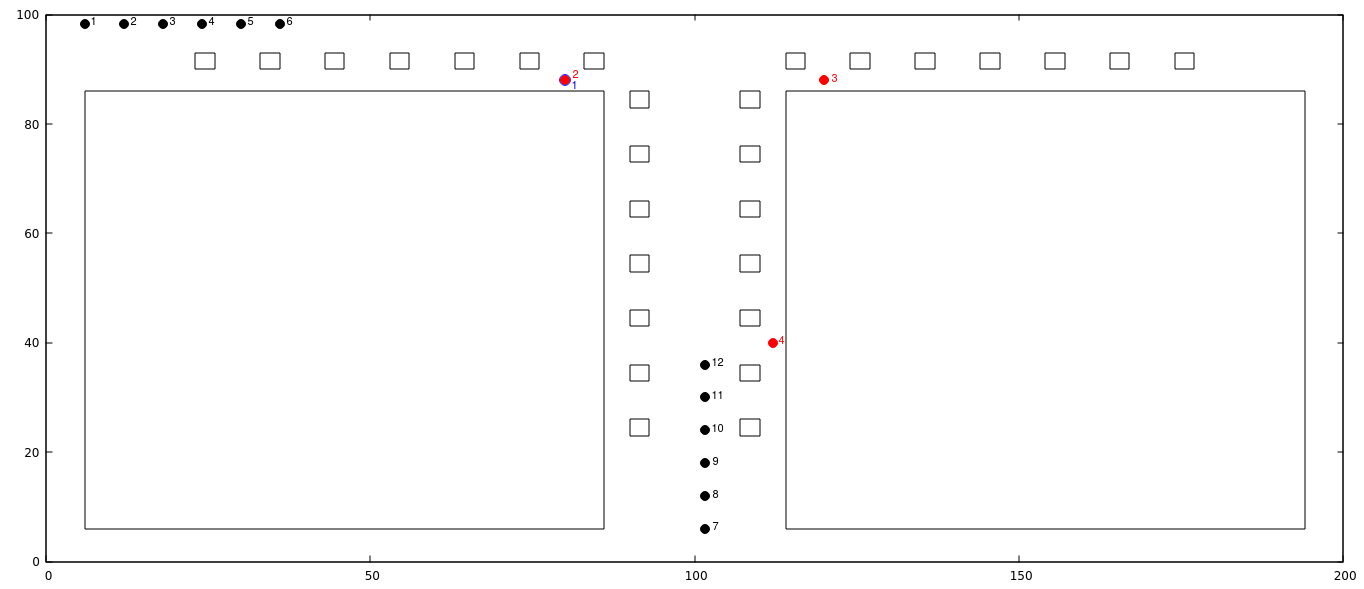
\includegraphics[width=14cm]{images/scenario.eps}
		\caption{The scenario as it was built using SUMO and ns-3. Red dots represent the mmWave eNBs and black dots are the UEs. Squares and rectangles represent the buildings: the small ones at the side of the road were used to simulate the presence of trees. Horizontal and vertical axes represent distance in meters.}
		\label{fig:scenario}
	\end{center}
\end{figure*}

The construction of the simulation scenario consists of two phases: the construction of the urban environment generating the speed and position traces of the vehicles and the usage of the traces to build the network using the ns-3 simulator. In the first phase we used a tool called SUMO \cite{} that allows to set up of a vast variety of urban traffic situations. 
Our choice was to keep the environment simple, while not sacrificing a minimum amount of complexity that is required to make the mmWave connectivity as challenging as it could be in a real urban vehicular environment. For this reason we reproduced a crossroad shaped as a "T" with traffic lights in the middle and two car flows coming from the bottom and left roads. We decided to use a small but reasonable number of cars to effectively simulate a real situation, 12, that are divided into 2 groups of 6 that enter the simulation respectively from the left road and the bottom road. The parameters we could set with SUMO are many, but the important ones in terms of the kind of simulation we performed are the length to the roads that is 200 m for the horizontal one and 100 m for then vertical one (so these are the maximum distances we are dealing with in the scenario), the length of the vehicles was set to 4 m for all of them and their speed is randomly chosen for each one and varies during the simulation but is limited to the interval $[0, 13.8]$ m/s.
The total duration of the simulation in the SUMO environment is 60 seconds, during which the semaphore acts only on the flow coming from the left that therefore enters the scenario and stops before the crossroad; the bottom flow is instead allowed to pass and all of its 6 vehicles enter the crossroad and turn right, exiting the simulation after having completed the about 100 m that separate them from the end of the road. After about 45 s, the traffic light lets the left flow pass too and 3 cars turn right in the bottom road while the other 3 go straight on. After 60 s all the cars have exited the scenario and passed through the crossroad. The output of the SUMO simulation is a file containing the position and velocity traces of all the 12 vehicles during the simulation, that we could import in the ns-3 simulator to generate a network in which nodes moved with respect to the base stations as cars did in the crossroad just described. 

Ns-3 is a open-source network simulator, developed in C++, that implements a vast number of protocols and channel models and that can be particularly useful in the simulation of cross-layer performances of protocols or network solutions. University of Padua and the New York University recently developed a mmWave module for ns-3 that is extensively described in \cite{e2esim} and that we used to realize the vehicular network we wanted to analyze. In particular, using a tool called \texttt{MobilityHelper}, ns-3 allows to import the mobility traces realized with SUMO and to create a network in which the mmWave UEs are cars with realistic speed and position. In addition to the UEs, to create a network we need the base station that can coordinate and provide traffic to the nodes: we used 4 base stations, 3 of them mmWave eNBs and one LTE eNB that act as link towards the Internet and serves as coordinator for the handover procedures. The scenario realized in ns-3 is shown in figure \ref{fig:scenario}.

As it can be seen in the figure, UEs are represented with black numbered dots and they are ordered in the same sequence they will enter the simulation. The 4 eNBs are instead represented by the red dots and one of them, number 4, serves as both a mmWave station and the LTE station. Rectangles represent buildings, that ns-3 allows to reproduce to simulate blockage and reflection that is common in real wireless networks. We decided to add to the scenario two buildings to make the environment more similar to a modern city and many small buildings at the side of the road to simulate the presence of trees and make the connectivity more difficult for the mmWave eNBs that many times cannot connect to the UEs in line of sight condition (LOS).
The details regarding the position of the buildings, the eNBs and trees can be found in table \ref{tab:envdetails}.

\begin{table*}[htbp]
	\begin{center}
		\begin{tabular}{p{2.7cm}ccccc}
			\toprule
			& \multicolumn{5}{c}{\textbf{Scenario parameters [m]}} \\
			\cmidrule(lr){2-6}
			Element          & Coordinates (X,Y) & Base dimensions (X$\times$Y)& Height (Z) & Road dist. & eNB dist. \\
			\midrule
			Building (left)  & 6:86, 6:86        & $80\times80$                & 25         & 14         & 2\\
			Building (right) & 114:194, 6:86     & $80\times80$                & 25         & 14         & 2\\
			Trees            & spaced by 7       & $3\times3$                  & 5          & 10         & 2\\
			eNB 2            & 80, 88            & -                           & 3          & 12         & - \\
			eNB 3            & 120, 88           & -                           & 3          & 12         & - \\
			eNB 4            & 112, 40           & -                           & 3          & 12         & - \\

			\bottomrule
		\end{tabular}
	\end{center}
	\label{tab:envdetails}
	\caption{The scenario parameters expressed in meters. The coordinates for the buildings are expressed in the format Xstart:Xend,Ystart:Yend, while for the trees we omit the coordinates of each tree and instead indicate the distance between a tree and the next one.}
\end{table*} 

\noindent As we can see there are some parameters that deserve some attention. First of all the distances have been chosen to be as realistic as possible, respecting however some constraints imposed by the network simulator. Indeed a rule that one must respect in setting up a network scenario in ns-3 is that the UE can not be too near to the base station, and the minimum distance they must keep is 10 m. For this reason the eNB are bound to be positioned at least 10 m away from the street in such a way that moving towards the crossroad they do not violate this rule. 
Also, we needed to ensure that both trees and buildings are realistically positioned and that they provide some level of blockage being between a car and a eNB in some moments of the simulation.

Once the scenario was set up, the actual network had to be created: the 12 nodes and 4 stations must be able to exchange packets and traffic with the Internet. The networking side of the model was built using the tool \texttt{MmWaveHelper}, that allows to create nodes that can provide mmWave connectivity, simulating the channel and all the required protocols, included the X2 protocol for the communication between the LTE station and the other eNBs \cite{e2esim}. The maximum rate that can be achieved with the kind of mmWave eNBs used is 3 Gb/s. At the same time, with the standard ns-3 LTE module we also set up the LTE station that occupies the same position as the mmWave eNB 4. To provide connectivity to the base stations, the tools \texttt{PointToPointHelper} and \texttt{MmWavePointToPointEpcHelper} create the core network through a gateway and a remote host that combined are used to simulate the Internet outside our network scenario \cite{e2esim}. Ns-3 also has tools to create the Internet stack, that in our case consists of IP addressing and UDP configuration, and to install it on nodes. 
The \texttt{MobilityHelper} was used to provide mobility to the created nodes according to the traces of the SUMO simulation. An application layer simulator present in ns-3 was finally what guaranteed the exchange of UDP packets between the nodes and the Internet: every UE starts an application that requires a UDP packet every 1$\mu$s. This application is able to saturate the eNBs, putting them in the correct state to analyze the maximum throughput achievable in a real time situation. Packets forwarded by the stations have a size of 1054 bytes. 

The network created in this way was what we used to test our proposed handover procedures: in the next section are presented the three different methods that we developed and a few words are spent about their implementation in the ns-3 LTE RRC model.
 

\subsection{Methods to improve the handover QoS metrics}

The handover procedure described in section \ref{sec:symohand} has its core in the criterion used by the LTE coordinator station, that has all the informations on the situation of the received SINR of all UEs, to decide when a UE has to switch between two base stations. The standard rule implemented in ns-3 is the one used nowadays by LTE cellular networks (we will refer to it as DHO in the following analysis) and consists in \cite{imphand}:

\begin{itemize}
	\item The coordinator monitors the received SINR by an UE from all the eNBs.
	\item Whenever a eNB (target cell) different from the one the UE is actually connected to provides a SINR higher than the present eNB by more than 3 dB, the coordinator keeps track of the difference between the two SINRs for a time equal to TTT seconds (time-to-trigger).
	\item If the new eNB keeps providing a better SINR by more than 3dB for all the duration of the TTT, the coordinator orders the switch of the UE to the new eNB.
\end{itemize}

In \cite{imphand} the authors even analyze two different ways to choose the TTT value: one is to keep it fixed at, for example, $f_{TTT}=150ms$, and the other to have a \emph{dynamic} threshold that is higher if the difference $\Delta$ between the current eNB SINR and the target is smaller. 

\subsubsection{Methods 1-2}
In the first and second policies we propose the procedure is similar. We base the handover criterion on a threshold for the received SINR from the target eNB, that we will call SINR*:

\begin{itemize}
	\item The coordinator keeps track of the maximum SINR received for each UE.
	\item If there are SINRs from one or more eNBs that are close to the maximum one, in the sense that the difference between the two is lower than the threshold SINR*, the coordinator triggers the handover towards the eNB that has the lowest number of UEs connected to it among those with SINR inside the threshold.
	\item If there are no other stations that provide a SINR that has a distance from the maximum lower than SINR* than the UE remains connected to the current base station that provides the maximum SINR.
\end{itemize}

The aim of this method is to take into account the fact that the throughput and the delay of the connection in a urban mmWave scenario may strongly depend on the congestion of the eNBs due to the excessive number of vehicles connected. For this reason, considering that the better SINR is not always an index of better connectivity but taking into account the fact that the target eNB may be overloaded may provide an improvement over the standard procedure. Indeed the SINR only takes into account, for the handover decision, path-loss, blockage and in general the quality of the channel without considering the number of resources the eNB is currently handling.

The key point is in how to choose the value for SINR*. We propose two different approaches: a static value equal to SINR*$=20$ dB, and a dynamic value where the threshold SINR* is chosen equal to the average of the received SINRs from the three mmWave eNBs. In the next sections we will refer to these two methods with MHO100 and MHOM (Modified HandOver 100 and Modified HandOver Mean).

\subsubsection{Method 3}
 In the third method we tried a different approach. The aim this time was to maximize the capacity of the channel used by the UEs, trying to take into account the congestion by means of the Shannon formula for channel capacity. Indeed, the channel capacity offered by a base station $i$ can be approximately expressed as:
 $$
 C_i=\frac{1}{N_i} B \log(1+SINR_i)
 $$
\noindent where $N_i$ is the number of UEs connected to the eNB because the capacity has to be shared among all the nodes connected, $B$ is the channel bandwidth and $SINR_i$ is the received SINR from the base station $i$. 
The proposed policy is the following:

\begin{itemize}
	\item The UE is initially connected to the eNB $i$.
	\item The coordinator triggers the handover towards the eNB $j$ if:
	$$
	\frac{1}{N_i} \log(1+SINR_i) < \frac{1}{N_j+1} \log(1+SINR_j)
	$$ 
\end{itemize}
\noindent that is if the channel capacity offered by the target base station is higher than the current one. Notice that the bandwidth can be simplified form the expression and that $N_j$ has to be incremented by one to take into account that if the handover is performed the target eNB will have one more UE to serve.

%%%%%%%%%%%%%%%%%%%%%%%%%%%%%%%%%%%%%%%%%%%%%%%
\section{Results}\label{sec:res}
%%%%%%%%%%%%%%%%%%%%%%%%%%%%%%%%%%%%%%%%%%%%%%%
The Results section contains a selection of the most relevant results with the explanation of their meaning. Please, not that you do NOT have to describe the shape of the curves that can be seen in the figures, but the reasons WHY such curves have that shape!

%%%%%%%%%%%%%%%%%%%%%%%%%%%%%%%%%%%
\section{Conclusions}\label{sec:conclusion}
%%%%%%%%%%%%%%%%%%%%%%%%%%%%%%%%%%%
Conclusions are a superbrief summary of what has been done and highlighting of the "take home message"



\addtocontents{toc}{Bibliografia}
\begin{thebibliography}{15}
	
	\bibitem{surveh}
	V. Va, T. Shimizu, G. Bansal, R. W. Wealth Jr et al.,
	\textit{Millimiter Wave vehicular communications: a survey}. 
	Foundations and trends in Networking, vol. 10, no. 1, 2016..
	
	\bibitem{mmvehicle}
	M. Giordani, A. Zanella, M. Zorzi,
	\textit{Millimiter Wave Communication in Vehicuar Networks: Challenges and Opportunities}. 
	IEEE 6th International Conference on Modern Circuits and System Technologies, 2017.
	
	\bibitem{imphand}
	M. Polese, M. Giordani, M. Mezzavilla, S. Rangan, M. Zorzi,
	\textit{Improved Handover Through Dual Connectivity in 5G mmWave Mobile Networks}. 
	IEEE Journal on Selected Areas in Communications, vol. 35, no. 9, pp. 2069-2084, 2017.
	
	\bibitem{e2esim}
	M. Mezzavilla, M. Zhang, M. Polese, R. Ford, S. Dutta, S. Rangan, M. Zorzi,
	\textit{End-to-End Simulation of 5G mmWave Networks}. 
	arXiv preprint, 2017.
	
	\bibitem{mmwwicom}
	T. S. Rapparport, R. W: Heath Jr, R. C. Daniels, J.N. Murdock,
	\textit{Millimeter Wave Wireless communications}.
	Prentice Hall, 2015.
	
	\bibitem{mmwcomsy}
	K. C. Huang, P. Rapajic, Z. Wang
	\textit{Millimiter Wave Communication Systems}.
	Wiley, 2011.
	
	\bibitem{mmwpac}
	S. Rangan, T. S. Rappaport, E. Erkip,
	\textit{Millimiter-Wave Cellular Wireless Netwoeks: Potentials and Challenges}
	Proceedings of the IEEE, vol. 102, no. 3, March 2014
	
\end{thebibliography}

\end{document}
